\documentclass{article}[11pt]

\usepackage{amsmath}
\usepackage{amssymb}
\usepackage{nicefrac}

\usepackage{pdflscape}

\usepackage{upgreek}

\usepackage{bashful}

% No intendation
\setlength\parindent{0pt}

\usepackage{hyperref}

\usepackage{siunitx}
\sisetup{
  per-mode=fraction,
  fraction-function=\tfrac
}

\usepackage{listings}
  \lstset{
    basicstyle=\ttfamily,
    escapeinside=||,
    xleftmargin=1cm
  }

\usepackage{float}

\usepackage{longtable}

\usepackage{multirow}

\usepackage{tikz}
  \usetikzlibrary{patterns}
  \usetikzlibrary{arrows.meta}
  \usetikzlibrary{shapes.misc}
  \usetikzlibrary{calc}

\usepackage{pgfplots}

\usepackage{cleveref}
\crefmultiformat{equation}{(#2#1#3)}{ and~(#2#1#3)}{, (#2#1#3)}{ and~(#2#1#3)}


\usepackage{acronym}
\usepackage[acronym,nonumberlist]{glossaries}
\glsdisablehyper
\makeglossaries
\newacronym{spice}{SPICE}{Simulation Program with Integrated Circuit Emphasis}
\newacronym{lef}{LEF}{Library Exchange Format}
\newacronym{dft}{DFT}{Discrete Fourier Transform}
\newacronym{dtft}{DTFT}{Discrete-Time Fourier Transform}
\newacronym{fft}{FFT}{Fast Fourier Transform}
\newacronym{mosfet}{MOSFET}{Metal–Oxide–Semiconductor Field-Effect Transistor}
\newacronym{clm}{CLM}{Channel Length Modulation}
\newacronym{de}{DE}{differential equation}
\newacronym{soi}{SOI}{silicon-on-insulator}
\newacronym{ldo}{LDO}{low-dropout regulator}
\newacronym{ota}{OTA}{operational-transconductance amplifier}
\newacronym{ofa}{OFA}{operational-floating amplifier}

% literature
\usepackage[ backend=biber
           , isbn=true
           , sorting=none
           , style=ieee
           ]{biblatex}
\addbibresource{./../../literature.bib}

% definitions
\def \whatis       {Notes}
\def \title        {Fuubar}

\def \author       {Matthias Schweikardt}

\def \authorMail   {mschweikardt@posteo.de}

\def \authorGithub {mschweikardt}

\def \license      {CC BY-SA 4.0}
\def \licenseUrl   {https://creativecommons.org/licenses/by-sa/4.0/}

\def \date         {nodate}

\def \pdfurl       {https://mschweikardt.github.io/ee-notes/%
\bash[stdout]
IFS=/ 
var=($PWD)
echo ${var[-1]}
\END%
.pdf
}
\def \srcurl       {srcurl}


% Customize footer and header of document
\usepackage{fancyhdr}

% Access last page number
\usepackage{lastpage}

% Access last page number
\usepackage[thinc]{esdiff}

% Physics
\usepackage{physics}

% Comment environment
\usepackage{comment}

% Subcaptions
\usepackage{subcaption}

% Thicker lines in tables
\usepackage{booktabs}

% Indentation in footnote
\makeatletter
\renewcommand\@makefntext[1]{\leftskip=2em\hskip-0.5em\@makefnmark#1}
\makeatother         

% qty with the siunitx definition
\AtBeginDocument{\RenewCommandCopy\qty\SI}

% TikZ compatibility
\pgfplotsset{compat=1.18}


\makeatletter
\pgfmathdeclarefunction{myatan2}{2}{%
\begingroup%
  \pgfmathfloattofixed{#1}\edef\tempa{\pgfmathresult}%
  \pgfmathfloattofixed{#2}%
  \pgfkeys{pgf/fpu=false}%
  \pgfmathparse{atan2(\tempa,\pgfmathresult)}\pgfkeys{/pgf/fpu}%
  \pgfmathfloatparsenumber{\pgfmathresult}%
  \pgfmath@smuggleone\pgfmathresult%
\endgroup
}
\makeatother

\usepackage{tabularx}
\usepackage{amsmath}
\usepackage{amssymb}
\usepackage{nicefrac}

\usepackage{pdflscape}

\usepackage{upgreek}

\usepackage{bashful}

% No intendation
\setlength\parindent{0pt}

\usepackage{hyperref}

\usepackage{siunitx}
\sisetup{
  per-mode=fraction,
  fraction-function=\tfrac
}

\usepackage{listings}
  \lstset{
    basicstyle=\ttfamily,
    escapeinside=||,
    xleftmargin=1cm
  }

\usepackage{float}

\usepackage{longtable}

\usepackage{multirow}

\usepackage{tikz}
  \usetikzlibrary{patterns}
  \usetikzlibrary{arrows.meta}
  \usetikzlibrary{shapes.misc}
  \usetikzlibrary{calc}

\usepackage{pgfplots}

\usepackage{cleveref}
\crefmultiformat{equation}{(#2#1#3)}{ and~(#2#1#3)}{, (#2#1#3)}{ and~(#2#1#3)}


\usepackage{acronym}
\usepackage[acronym,nonumberlist]{glossaries}
\glsdisablehyper
\makeglossaries
\newacronym{spice}{SPICE}{Simulation Program with Integrated Circuit Emphasis}
\newacronym{lef}{LEF}{Library Exchange Format}
\newacronym{dft}{DFT}{Discrete Fourier Transform}
\newacronym{dtft}{DTFT}{Discrete-Time Fourier Transform}
\newacronym{fft}{FFT}{Fast Fourier Transform}
\newacronym{mosfet}{MOSFET}{Metal–Oxide–Semiconductor Field-Effect Transistor}
\newacronym{clm}{CLM}{Channel Length Modulation}
\newacronym{de}{DE}{differential equation}
\newacronym{soi}{SOI}{silicon-on-insulator}
\newacronym{ldo}{LDO}{low-dropout regulator}
\newacronym{ota}{OTA}{operational-transconductance amplifier}
\newacronym{ofa}{OFA}{operational-floating amplifier}

% literature
\usepackage[ backend=biber
           , isbn=true
           , sorting=none
           , style=ieee
           ]{biblatex}
\addbibresource{./../../literature.bib}

% definitions
\def \whatis       {Notes}
\def \title        {Fuubar}

\def \author       {Matthias Schweikardt}

\def \authorMail   {mschweikardt@posteo.de}

\def \authorGithub {mschweikardt}

\def \license      {CC BY-SA 4.0}
\def \licenseUrl   {https://creativecommons.org/licenses/by-sa/4.0/}

\def \date         {nodate}

\def \pdfurl       {https://mschweikardt.github.io/ee-notes/%
\bash[stdout]
IFS=/ 
var=($PWD)
echo ${var[-1]}
\END%
.pdf
}
\def \srcurl       {srcurl}


% Customize footer and header of document
\usepackage{fancyhdr}

% Access last page number
\usepackage{lastpage}

% Access last page number
\usepackage[thinc]{esdiff}

% Physics
\usepackage{physics}

% Comment environment
\usepackage{comment}

% Subcaptions
\usepackage{subcaption}

% Thicker lines in tables
\usepackage{booktabs}

% Indentation in footnote
\makeatletter
\renewcommand\@makefntext[1]{\leftskip=2em\hskip-0.5em\@makefnmark#1}
\makeatother         

% qty with the siunitx definition
\AtBeginDocument{\RenewCommandCopy\qty\SI}

% TikZ compatibility
\pgfplotsset{compat=1.18}


\makeatletter
\pgfmathdeclarefunction{myatan2}{2}{%
\begingroup%
  \pgfmathfloattofixed{#1}\edef\tempa{\pgfmathresult}%
  \pgfmathfloattofixed{#2}%
  \pgfkeys{pgf/fpu=false}%
  \pgfmathparse{atan2(\tempa,\pgfmathresult)}\pgfkeys{/pgf/fpu}%
  \pgfmathfloatparsenumber{\pgfmathresult}%
  \pgfmath@smuggleone\pgfmathresult%
\endgroup
}
\makeatother

\usepackage{tabularx}


\def \title  {Pole-Zero Doublet}
\def \date   {May 16, 2025}

\def \pdfurl {https://mschweikardt.github.io/ee-notes/pole-zero-doublet.pdf}
\def \srcurl {https://github.com/mschweikardt/ee-notes/tree/main/notes/pole-zero-doublet}

\usepackage[scale=5]{draftwatermark}

\begin{document}

\notetitle

\begin{equation}\label{eq:fs}
\underline{F}(j\omega) = \frac{1+\frac{j\omega}{\omega_{\mathrm{z}}}}{1+\frac{j\omega}{\omega_{\mathrm{p}}}}
\end{equation}

\begin{equation}
\omega_{\mathrm{p}} > \omega_{\mathrm{z}} > 0
\end{equation}

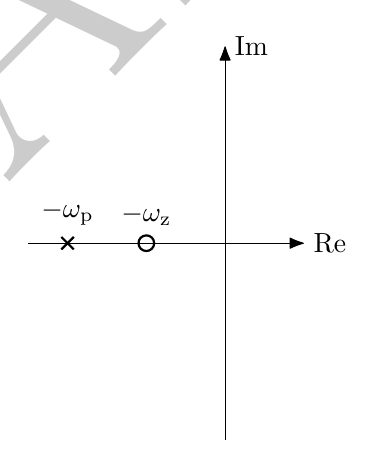
\begin{tikzpicture}[scale=1.0]
  \draw[-{Latex[round,scale=1.2,round]}] (-2.5,0) -- (1,0);
  \node[anchor=west] at (1,0) {Re};
  \draw[-{Latex[round,scale=1.2,round]}] (0,-2.5) -- (0,2.5);
  \node[anchor=west] at (0,2.5) {Im};

  \node[cross out,draw=black,thick,scale=0.6] at (-2, 0) {};
  \node[circle,draw=black,thick,scale=0.6] at (-1, 0) {};
  \node[anchor=south] at (-2, 0.1) {$-\omega_{\mathrm{p}}$};
  \node[anchor=south] at (-1, 0.1) {$-\omega_{\mathrm{z}}$};
\end{tikzpicture}

\begin{equation}
\begin{split}
\arg\left(\underline{F}(j\omega)\right) &= \arctan\left(\frac{\omega}{\omega_{\mathrm{z}}}\right) - \arctan\left(\frac{\omega}{\omega_{\mathrm{p}}}\right) \\
                                        &= \arctan\left(\frac{\omega}{\omega_{\mathrm{z}}}\right) - \arctan\left(\frac{\omega_{\mathrm{z}}}{\omega_{\mathrm{p}}} \frac{\omega}{\omega_{\mathrm{z}}}\right)
\end{split}
\end{equation}

\begin{equation}
\delta = \frac{\omega_{\mathrm{p}}}{\omega_{\mathrm{z}}}
\end{equation}

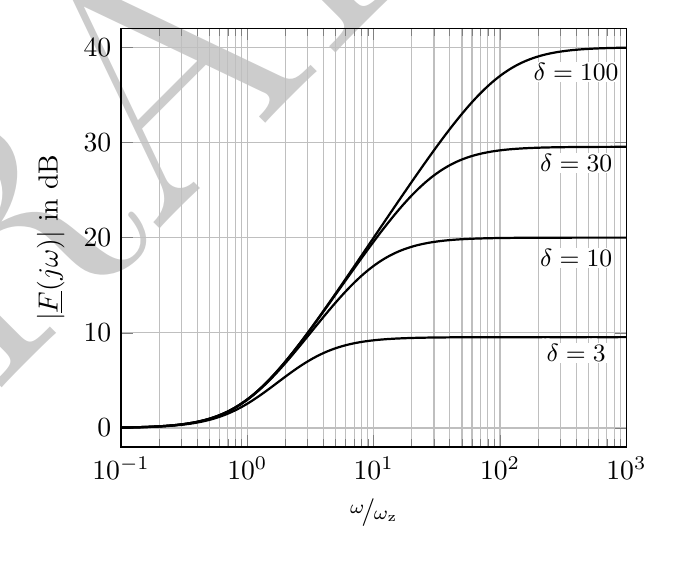
\begin{tikzpicture}
  \begin{axis}[ ylabel=$\left|\underline{F}(j\omega)\right|$ in \si{\decibel}
              , xlabel=$\nicefrac{\omega}{\omega_{\mathrm{z}}}$
              , xmode=log
              , ymin=-2
              , ymax=42
              , xmin=0.1
              , xmax=1000
              , grid=both
              , width=8cm
              ]

     \addplot[ domain=0.001:1000
             , samples=301
             , smooth
             , thick] {20*log10(sqrt(1+x^2))-20*log10(sqrt(1+(x/3)^2))};             
     \addplot[ domain=0.001:1000
             , samples=301
             , smooth
             , thick] {20*log10(sqrt(1+x^2))-20*log10(sqrt(1+(x/10)^2))}; 
     \addplot[ domain=0.001:1000
             , samples=301
             , smooth
             , thick] {20*log10(sqrt(1+x^2))-20*log10(sqrt(1+(x/30)^2))};
     \addplot[ domain=0.001:1000
             , samples=301
             , smooth
             , thick] {20*log10(sqrt(1+x^2))-20*log10(sqrt(1+(x/100)^2))}; 

      \node[anchor=north,font=\small,fill=white,inner sep=0.5pt] 
        at (axis cs:400,9) {$\delta=3$};
      \node[anchor=north,font=\small,fill=white,inner sep=0.5pt] 
        at (axis cs:400,19) {$\delta=10$};
      \node[anchor=north,font=\small,fill=white,inner sep=0.5pt] 
        at (axis cs:400,29) {$\delta=30$};
      \node[anchor=north,font=\small,fill=white,inner sep=0.5pt] 
        at (axis cs:400,38.5) {$\delta=100$};
  \end{axis}
\end{tikzpicture}
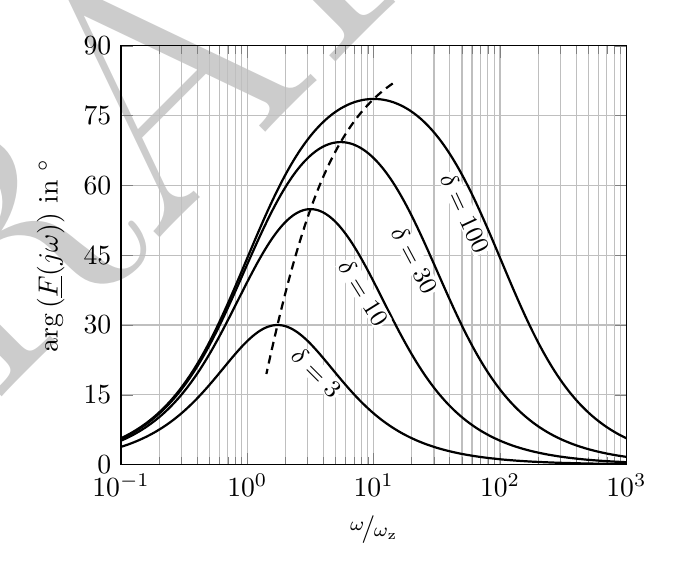
\begin{tikzpicture}
  \begin{axis}[ ylabel=$\arg\left(\underline{F}(j\omega)\right)$ in \si{\degree}
              , xlabel=$\nicefrac{\omega}{\omega_{\mathrm{z}}}$
              , xmode=log
              , ymin=0
              , ymax=90
              , xmin=0.1
              , xmax=1000
              , grid=both
              , width=8cm
              , ytick={0,15,...,90}
              ]

     \addplot[ domain=0.001:1000
             , samples=301
             , smooth
             , thick] {atan(x)-atan(x/3)}; 
     \addplot[ domain=0.001:1000
             , samples=301
             , smooth
             , thick] {atan(x)-atan(x/10)}; 
     \addplot[ domain=0.001:1000
             , samples=301
             , smooth
             , thick] {atan(x)-atan(x/30)}; 
     \addplot[ domain=0.001:1000
             , samples=301
             , smooth
             , thick] {atan(x)-atan(x/100)}; 

     \addplot[ domain=0.005:0.5
             , samples=301
             , smooth
             , densely dashed
             , thick] ({1/sqrt(x)},{atan(1/sqrt(x))-atan(sqrt(x))}); 

      \node[anchor=east,font=\small,fill=white,inner sep=0.5pt,rotate=-45] 
        at (axis cs:5.3,15) {$\delta=3$};
      \node[anchor=east,font=\small,fill=white,inner sep=0.5pt,rotate=-58] 
        at (axis cs:12,30) {$\delta=10$};
      \node[anchor=north,font=\small,fill=white,inner sep=0.5pt,rotate=-62] 
        at (axis cs:25,45) {$\delta=30$};
      \node[anchor=north,font=\small,fill=white,inner sep=0.5pt,rotate=-65] 
        at (axis cs:63,55) {$\delta=100$};
  \end{axis}
\end{tikzpicture}

Peak of phase at
\begin{equation}
\frac{\omega_{\mathrm{p}}}{\omega_{\mathrm{z}}} = \sqrt{\delta}
\end{equation}
with
\begin{equation}
\arg\left(\underline{F}(j\omega)\right) = 
  \arctan\left(\sqrt{\delta}\right)-\arctan\left(\frac{1}{\sqrt{\delta}}\right)
\end{equation}

\printbibliography

\end{document}